\newpage 
\appendix

\section{Center computation.}
\begin{algorithm}
    \caption{Find the centers of given radius which circumference laid on the two input points.}
    \begin{algorithmic}[1]
        \Require Radius $\frac{\varepsilon}{2}$ and points $p_1$ and $p_2$.
        \Ensure Centers $c_1$ and $c_2$.
        
        \Function{FindCenters}{$p_1$, $p_2$, $\frac{\varepsilon}{2}$}
        \State $r^2 \gets (\frac{\varepsilon}{2})^2$
        \State $X \gets p_1.x - p_2.x$
        \State $Y \gets p_1.y - p_2.y$
        \State $d^2 \gets X^2 + Y^2$
        \State $R \gets \sqrt{\lvert 4 \times \frac{r^2}{d^2} - 1 \rvert}$
        \State $c_1.x \gets X + \frac{Y \times R}{2} + p_2.x$
        \State $c_1.y \gets Y - \frac{X \times R}{2} + p_2.y$
        \State $c_2.x \gets X - \frac{Y \times R}{2} + p_2.x$
        \State $c_2.y \gets Y + \frac{X \times R}{2} + p_2.y$
        
        \State \Return $c_1$ and $c_2$
        \EndFunction
    \end{algorithmic}
    \label{app:centers}
\end{algorithm}

\section{Disk pruning.}
\begin{algorithm}
    \caption{Prune disks which are duplicate or subset of others.}
    \begin{algorithmic}[1]
        \Require Set of disks $D$.
        \Ensure Set of disks $D^{\prime}$ without duplicate or subsets.
        
        \Function{PruneDisks}{$D$}
        \State $E \gets \varnothing$
        \ForAll{disk $d_i$ in $D$}
            \State $N \gets d_i \cap D$
            \ForAll{disk $n_j$ in $N$}
                \If{$d_i$ contains all the elements of $n_j$}
                        \State $E \gets E \cup {n_j}$
                \EndIf
            \EndFor
        \EndFor        
        \State $D^{\prime} \gets D \setminus E$
        \State \Return $D^{\prime}$
        \EndFunction
    \end{algorithmic}
    \label{app:disks}
\end{algorithm}

\section{Clique and MBC approach.}
\begin{figure}
    \centering
    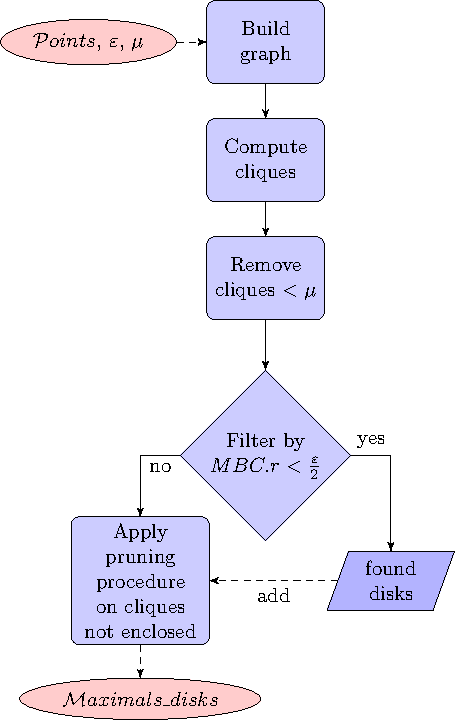
\includegraphics[width=0.7\linewidth]{figures/plots/10_cmbc_variants/CMBC_flowchart2.pdf}
    \caption{Schematic description of the Clique and MBC approach.}
    \label{fig:cmbc_flowchart}
\end{figure}